\pling\ is a portfolio-based SAT solver... [[Short explanation of plingeling]]

\subsection{Modified \pling}
\label{sec:modifiedpling}


One of the advantages we assume of parallel computing is that the more
cores we add, the better performance we will obtain. This should be
also true for \pling, since the only difference of adding more threads
(assuming we have one thread per core) is that we will have a greater
variety of solver strategies trying to solve the same problem, and
also some logical clause sharing among threads. These are all valid
assumptions in theory, but empirical results on multicore shared
memory computers also show us that increasing the number of threads
also carries a considerable decrease in performance for portfolio
solvers like {\tt plingeling}.


Multicore shared memory systems have their cores sharing the same last
level cache (LLC) memory. The last level cache size in modern machines
has a few megabytes and is usually not enough to hold all the data
required by a SAT instance. Therefore, there will inevitably be some
communication between the LLC and the main memory. The time cost of
communications between the CPU and the LLC cache are much faster than
having to get the data from main memory, so we would like to keep data
transfers from main memory to a minimum.

Portfolio SAT solvers which only share clauses logically have to keep
a complete database of clauses for each thread's use. So as we add
more threads, the solver has greater needs of memory, but because all
cores share the same LLC, all threads will have a lower chance of
finding their data in the LLC as we add more threads. In this
scenario, what we would expect is to observe, as we have in our
experiments, a considerable decrease in performance when adding
threads, simply because we will incur in more LLC cache misses when
the amount of data to be manipulated by different threads
increases. We don't usually appreciate this negative performance
impact in these type of solvers, because different threads implement
different SAT solving strategies, so the solving time will mostly
depend on the fastest solving thread, shadowing the negative
performance impact of copying the clause database in each thread. 

In our experiments, we modified \pling to replicate the exact same
search in each of its threads. What we would expect, theoretically, is
that adding more threads would have no impact in the solving time,
because all cores would be making the exact same search with their own
data. However, in practice, we found that the performance decrease of
having six threads in six cores to be of around 15-40\% of the total
time one thread would take (Figure \ref{fig:decay}). The reasons for
this behavior may be due to several factors in modern SMP
architectures. However, sharing resources (such as the caches,
communication and/or synchronization, main memory) could be seen as
the main suspects. To find out what was happening in the machine, we
ran another experiment, where a \pling\ instance performing the same
search with four threads was executed on different CPU chips, and, to
compare, we ran the same experiment on four cores of the same CPU
chip.

% Because each CPU has its own LLC
% cache, we would expect in this case to have equal performance when
% running one thread compared to running four threads, which is what was
% observed in our measures.

[[EXPLAIN MODIFICATIONS]]

\begin{figure}
  \begin{center}
    \subfloat[on same
    chip]{\label{fig:4coressame}\includegraphics[bb=59 90 294 325,
      clip, width=0.5\textwidth]{plingeling_same_chip}} \subfloat[on
    different chips]{\label{fig:4coresdiff}\includegraphics[bb=59
      90 294 325, clip,
      width=0.5\textwidth]{plingeling_different_chip}}
    \caption{Modified \pling\ performance decay}
  \end{center}
\end{figure} 

As can be seen, executing the solver on {\em different} CPU chips does
not impact performance, while executing it on the {\em same} CPU chip
incurs in a significant performance decay. According to our experiment
above, the only shared resource that could impact performance when run
in one chip is the LLC or Last Level Cache. To effectively measure the
involvement of the LLC, we used the {\tt perf}
tool\footnote{\url{XXXXXX}} [[TALK ABOUT PERF]]

\begin{figure}[h]
  \centering
%  \includegraphics{}
  \caption{LLC statistics for modified \pling}
  \label{fig:LLCStats}  
\end{figure}

As the LLC-load-misses (number of times main memory data had to be
retrieved) figure (Figure \ref{fig:4coressame}) strongly suggests,
this performance decrease is due to the six thread solver wasting
much more time retrieving data from main memory
than its single threaded version did. As we would also expect, our
results show that the L1 cache behaves equally for each core, because
L1 caches are not shared as opposed to the LLC cache.

\subsection{\pling\ scalability}

In this section, we provide an overview of how \pling\ behaves at a
larger scale. So far, because of the experiment above, we know that
the more threads we add, the more the cache impacts negatively in
performance. However, we also know that adding threads also adds new
workers with new (and possibly successful) strategies. This results in
a trade-off between cache contention versus portfolio-approach
benefits. To test this, we ran the original \pling\ over 207 standard
benchmarks taken from past SAT races and competitions (see link
above), varying the number of threads from one to ten on a single chip
with 10 physical cores.

\begin{table}[h]
  \centering
  \begin{tabular}[h]{ccc}
    \hline
    {\bf Threads} & {\bf \# Problems solved} & {\bf Total time}\\
    \hline
    1&113&101399\\
    2&121&~95745\\
    3&119&~93854\\
    4&122&~90412\\
    5&124&~87953\\
    6&124&~89506\\
    7&127&~87416\\
    8&124&~88434\\
    9&124&~88931\\
    10&125&~89003\\
    \hline
    \hline
  \end{tabular}    
  \caption{Scalability}
  \label{tab:scal}
\end{table}


\begin{figure}[htp]
  \centering
  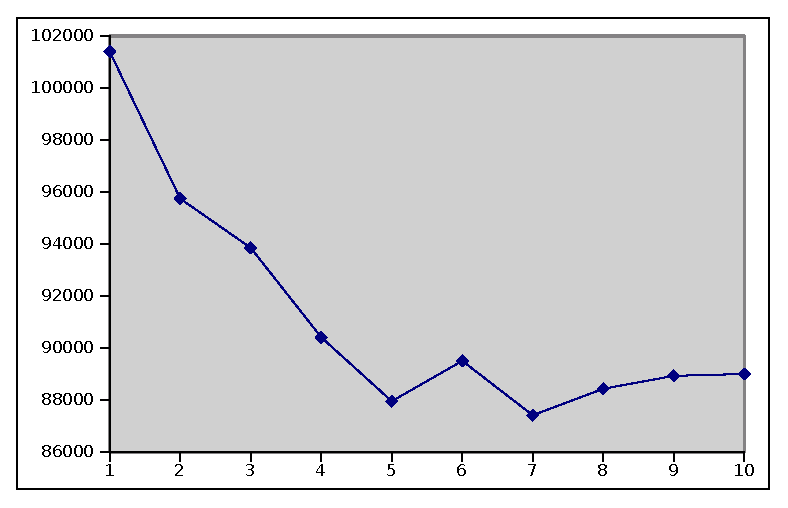
\includegraphics[scale=1]{plingperthread}
  \caption{Total solving time per number of threads.}
  \label{fig:pperfpthread}
\end{figure}

Figure \ref{fig:pperfpthread} and Table \ref{tab:scal} show that up
until the fifth thread, scalability is good, but from then on, the
number of solved problems and total time reaches a plateau. This means
that \pling\ cannot scale up on the number of cores sharing an LLC. 
%but it does scale on number of separate chips.

%%% Local Variables: 
%%% mode: latex
%%% TeX-master: "sat"
%%% End: 
